% \documentclass[10pt, a4paper]{amsart}
\documentclass[%
reprint,
nofootinbib,
%superscriptaddress,
%groupedaddress,
%unsortedaddress,
%runinaddress,
%frontmatterverbose,
%preprint,
%showpacs,preprintnumbers,
%nofootinbib,
%nobibnotes,
%bibnotes,
amsmath,amssymb,
aps,
%pra,
%prb,
%rmp,
%prstab,
%prstper,
%floatfix,
]{revtex4-1}
\usepackage[]{graphicx}
\usepackage{float}
\usepackage[]{hyperref}
\usepackage[]{physics}
\usepackage[]{listings}
\usepackage[T1]{fontenc}
\usepackage{color}
\usepackage[]{subcaption}
\usepackage[ruled,vlined]{algorithm2e}
\usepackage{amssymb, amsmath}

\definecolor{mygreen}{rgb}{0,0.6,0}
\definecolor{mymauve}{rgb}{0.58,0,0.82}

\newcommand\todo[1]{\textcolor{red}{#1}}

\lstset{ %
	backgroundcolor=\color{white},   % choose the background color; you must add \usepackage{color} or \usepackage{xcolor}
	basicstyle=\footnotesize,        % the size of the fonts that are used for the code
	breakatwhitespace=false,         % sets if automatic breaks should only happen at whitespace
	breaklines=true,                 % sets automatic line breaking
	captionpos=b,                    % sets the caption-position to bottom
	commentstyle=\color{mygreen},    % comment style
	deletekeywords={...},            % if you want to delete keywords from the given language
	escapeinside={\%*}{*)},          % if you want to add LaTeX within your code
	extendedchars=true,              % lets you use non-ASCII characters; for 8-bits encodings only, does not work with UTF-8
	frame=single,	                   % adds a frame around the code
	keepspaces=true,                 % keeps spaces in text, useful for keeping indentation of code (possibly needs columns=flexible)
	keywordstyle=\color{blue},       % keyword style
	language=c++,                    % the language of the code
	otherkeywords={*,...},           % if you want to add more keywords to the set
	rulecolor=\color{black},         % if not set, the frame-color may be changed on line-breaks within not-black text (e.g. comments (green here))
	showspaces=false,                % show spaces everywhere adding particular underscores; it overrides 'showstringspaces'
	showstringspaces=false,          % underline spaces within strings only
	showtabs=false,                  % show tabs within strings adding particular underscores
	stepnumber=2,                    % the step between two line-numbers. If it's 1, each line will be numbered
	stringstyle=\color{mymauve},     % string literal style
	tabsize=2,	                     % sets default tabsize to 2 spaces
}


\begin{document}
	
\title{Ordinary differential equations\\
	\normalsize{Building a model for the solar system} \\
	\hrulefill\small{ FYS3150: Computational Physics }\hrulefill}

\author{Sigurd Sandvoll Sundberg}\homepage{https://github.com/SigurdSundberg/FYS3150}

\affiliation{%
	Department of Geosciences, University of Oslo\\
}%

\date{\today}

\begin{abstract}%[0]
We studied systems of coupled differential equations relating to planetary motion of our Solar system and different aspects of these systems. Through an object oriented structure we find it easy to adapt and change our systems without any additional work, and can easily change different aspects of our system. Through the study of stability and timing for our implemented differential solvers, forward Euler and velocity-Verlet methods, we find that the velocity-Verlet method is the superior choice when it comes to simulating Hamiltonian systems, even at the cost of a slower run time. Through the study of the two body system consisting of the Sun and the Earth we find that the escape velocity through iterating over our system, is $8.8849$AU/year, a standard deviation of $0.01\%$ from the found analytical value of $2\pi$AU/year. From the study of an alteration of Newton's gravitational law, we find that as the exponent approaches $3$, we get a gradually more unstable orbit, and diverges as it passes 3. Studying a three body system, with the addition of Jupiter, we find little to no notable difference in the orbits using the actual bary center or the center of the Sun as bary centers when studying this system. Altering the mass of Jupiter by factors of 10 and 1000, we find that the system behaves as expected with a shifted center of mass. For the increase in mass by a factor of 10 we see that the motion of the system over the simulated time is stable. However when increasing the mass by a factor of 1000, the three body system is unstable. The Earth gets slung our of orbit. Simulating the entire Solar system we see that the addition of multiple planets does not change the stability of the system. Lastly, we confirm the results of the general relativity's prediction of the perihelion precession of Mercury. Where we find that the found value of $42.612''$, with a standard deviation of $0.9\%$, from the observed value of $43''$ of the perihelion precession, supports that the perihelion precession can primarily be explained by general relativity. 
\end{abstract}

\maketitle 

\section{Introduction} %1
Being able to describe our Solar system has been an interest of philosophers and physicists alike, from geocentric models to heliocentric models. All the way up until today's model where we describe large parts of our observable universe. Kepler was the first to describe the motion planetary motion and laid the groundwork for further developments within Astronomy. Later Isaac Newton developed his gravitational law for describing the interactions between two objects, and this was used to further develop the theory of planetary motion. The theory developed by Newton had some limitations however, we are only able to find general solutions to a limited subset of all problems, with systems of two bodies being the limit. 
With the development of computers, we where able to efficiently solve many body problems, such as simulation of our Solar system.

From Newton's gravitational law, when solving for many body problems, we quickly end up with sets of coupled differential equations. There exists many different types of algorithms for solving  coupled differential equations, however not all are fit to solving physical systems. Our scope of algorithms is thus primarily algorithms which preserve energy and angular momentum precisely. In this project we take a look at the velocity-Verlet algorithm and compare it to the simple forward Euler. 
Comparing the two algorithms, we first look at a simple system only consisting of the Earth-Sun system, compared floating point operations(FLOPs) and time used by the two algorithms. Before extending the problem to three-body system and finally doing a simulation of the entire Solar system. 

To simulate many body problems, we also discuss object orientation(OO) and the benefits of having programs which we can be written once and ran many times. We do not need to change our entire code base when adding more objects, we can simply add more bodies and keep simulating the system. Object orientation makes us able to simulate vastly different systems and test different properties of the systems. Along side being able to easily test our implementation easily with simple systems, and quickly extending them to many body systems which are of interest. 

Topics we will look at besides simulating the Solar system, is finding the escape velocity of Earth, study different forms of Newton's gravitational law, and lastly we take a look at one of the most important tests of general theory of relativity, Mercury's perihelion precession. 

In this article we start by going through the theory used, how the algorithms are implemented and properties of them. Before we start looking at simulations of different systems and the results from our simulations. Lastly we discuss our results and their implication, before concluding our work. 
\section{Theory} %1
\subsection{Differential Equations}%1
The force acting upon objects in our Solar System are governed by Newton's gravitational law, which states that the force acting between two objects is 
\begin{equation}
	\vec{F}_{ij} =  -G \frac{m_im_j}{\abs{r_{ij}}^2}\hat{r}_{ij}
\end{equation}
where 
\begin{enumerate}
	\item	$F_{ij}$ is the force applied on object i by object j.
	\item G is the gravitational constant.
	\item	$m_i$ and $m_j$ are respectively the masses of objects i and j. 
	\item $\abs{r_{ij}} = \abs{\vec{r_i} - \vec{r_j}}$ is the distance between j and i.
	\item	$\hat{r}_{ij} = \frac{\vec{r_i}-\vec{r_j}}{\abs{\vec{r_i} - \vec{r_j}}}$ is the unit vector from object j to i.
\end{enumerate}
We let the force act on the center of mass of the objects, and consider the objects to be point particles. 

The total force acting on an object in the Solar System is given by 
\begin{equation}
	\vec{F}_i = \sum_{i\neq j} \vec{F}_{ij}
\end{equation}

From Newton's second law of motion we have,
\begin{equation}
 \vec{F} = m\vec{a}.
\end{equation}
Using $\vec{F} = \vec{F}_{ij}$ we can derive that 
\begin{equation}
	\begin{split}
		\vec{a} = \frac{\vec{F}}{m}\\
		\frac{\partial^2 }{\partial t^2}\vec{r} = \frac{\vec{F}}{m}
	\end{split}
\end{equation}
As the $\vec{F}$ is dependent on the position $\vec{r}$, we are dealing with coupled partial differential equations. We can rewrite this as a set of coupled ordinary differential equations(ODE), 
\begin{equation}\label{eq:diff}
	\begin{split}
		\frac{\partial}{\partial t} \vec{v} = \vec{a}\\
		\frac{\partial}{\partial t} \vec{r} = \vec{v}
	\end{split}
\end{equation}
Knowing the position of all the objects in the Solar System we can find the force acting upon each object, and from this find their respective position over time, by solving this set of differential equations. 

\subsection{Escape Velocity} %1
We can find the escape velocity of Earth by using the law of conservation of energy. Knowing that the escape velocity, is the minimum velocity require to escape a planet's gravitation pull. We then have 
\begin{equation}
	E_{\text{Total before}} = E_{\text{Total after}}
\end{equation}
To find the escape velocity, we set the terms on the right-hand side(RHS) to zero, that is the energy of the Earth an infinite distance away from the Sun and at rest. 
We then have 
\begin{equation}
	E_{\text{Total Before}} = K_i + U_i > 0
\end{equation}
where $K_i$ and $U_i$ are the initial kinetic and potential energy of the Earth, respectively. 
We then have 
\begin{equation}
	K_i + U_i = \frac{1}{2}M_Ev_E^2 + \frac{-GM_EM_{\odot}}{r} > 0
\end{equation}
Inserting for quantities of AU for distance, masses in Sun masses and time period in year we have
\begin{equation}
	\begin{split}
		M_{E_\odot}v_E^2 - 8\pi^2\frac{M_{E_\odot}}{1 \text{AU}} &> 0 \\
		v_E^2 &> 8\pi^2 \\
		v_E &> 2\pi\sqrt{2}
	\end{split}
\end{equation}
For the Earth to be able to escape the orbit around the Sun starting 1 AU away, would need a initial velocity of $2\pi\sqrt{2}\text{AU}/\text{year} \sim 8.88576 \text{AU}/\text{year}$.

\subsection{Conservation of Total Energy and Angular Momentum} %1
In this project we study closed system, that is, the only forces acting on the planets in our system is the force from the planets themselves. The force acting between the planets is the gravitational force, which is conservative. For a system where we only have conservative forces, energy is conserved\cite{book}. To note, is that when using numerical methods, certain methods do not conserve energy, whilst others do. 

Looking at the total angular momentum of the system, $\vec{L}$, we know that this value is be conserved as we have no external forces acting on our system. One way of showing this is looking at Kepler's second law of planetary motion. It states that \textit{a planet sweeps out equal areas in equal times, that is, the area divided by time is constant.}\cite{UniPhys}

The definition of angular momentum is given by $\vec{L} = \vec{r} \times \vec{p}$, where $\vec{L}$ is the angular momentum, $\vec{r}$ is the position and $\vec{p}$ is the instantaneous linear momentum. Since the movement in a orbit can be considered elliptical, $\vec{p}$ is always tangent to the ellipse. We can split $\vec{p}$ into two parts, on radial and one perpendicular, which gives us 
\begin{equation}
	\vec{L} = \vec{r} \times \vec{p} = \vec{r}\times \left(\vec{p}_{\text{rad}} + \vec{p}_{\text{perp}}\right) = \vec{r} \times \vec{p}_{\text{rad}} + \vec{r} \times \vec{p}_{\text{perp}}.
\end{equation}
We can see that the first term on the right is zero, since $\vec{p}_{\text{rad}}$ is parallel to $\vec{r}$, which gives us 
\begin{equation}
	\vec{L} = \vec{r}\times\vec{p}_{\text{perp}} = rmv_{\text{perp}}
\end{equation}
Since the gravitational force is only acting in the radial direction, it cannot change the perpendicular velocity, thus angular momentum is conserved. 


\subsection{Relativistic Correction to Newton's Gravitational Law} %1

An important test of the general theory of relativity, is to compare the predicted perihelion precession of Mercury to the observed value. The observed value when only considering a two-body system consisting of the Sun and Mercury is 43''(43 arc seconds) per century, compared to the predicted value.

Closed elliptical orbits are a special feature to the Newtonian $1/r^2$ force. In general, any correction to the pure $1/r^2$ behaviour will lead to an orbit which is not closed, that is, after one complete orbit around the Sun, the planet will not be at exactly the same position as it started. 

We can think of Mercury's orbit around the Sun, to be that of an ellipse, whose orientation in space slowly rotates. That is if the correction is small enough, as each orbit will be almost the same as the classical ellipse. This relativistic correction gives the Newtonian gravitational force a new form
\begin{equation}
	F_G = \frac{GM_{\odot}M_{\text{Mercury}}}{r^2}\left[1 + \frac{3 l^2}{r^2c^2}\right]
\end{equation}
where $M_{\text{Mercury}}$ is the mass of Mercury, $r$ is the distance between Mercury and the Sun, $l = \abs{\vec{r}\times\vec{v}}$ is the magnitude of Mercury's orbital angular momentum per unit mass, and $c$ is the speed of light in vacuum. 
 
\section{Algorithms}%1
In order to find the position for all bodies as time evolves we need to solve a set of couple differential equations \ref{eq:diff} for each of the bodies at each time step. In our case for the solar system this set of couple differential equations is only possible to solve numerically. 

To start off we want to scale our equations from SI units to more appropriate units for the solar system, these are Astronomical Unit(AU) for length, years(yr) for time and sun masses for mass. By looking at the Earth-Sun system, and assuming circular motion\cite{1994A&A...282..663S}, we have
\begin{equation}
	F_{\text{Earth}} = G\frac{M_{\text{Earth}}M_{\odot}}{r^2} = M_{\text{Earth}}\frac{v^2}{r}
\end{equation}
This gives us 
\begin{equation}
	GM_{\odot} = v^2 r = (2\pi \text{AU}/\text{yr})^2 1\text{AU} = 4\pi^2\text{AU}^3/\text{yr}^2.
\end{equation}
Using Sun masses\footnote{$M_{\odot} = 1$, and all other masses scaled as $M_i / M_{\odot}$.}, we then have 
\begin{equation}
	 G = 4\pi^2\text{AU}^3/\text{yr}^2.
\end{equation}

Our discretization of our continuous differential equations are done as follows
\begin{equation}
	\begin{split}
		&x(t) \rightarrow x(t_i) \rightarrow x_i \in [x_0, x_1, \dots, x_i, \dots, x_{n-1}]\\
		&v(t) \rightarrow v(t_i) \rightarrow v_i \in [v_0, v_1, \dots, v_i, \dots, v_{n-1}]
	\end{split}
\end{equation}
and so on, where the initial values are known. If we know the initial time $t_0$ and the final time $t_{\text{max}}$, and the number of integration points $n$, we get the following expressions for $t_i$ 
\begin{equation}
	t_i = t_0 + hi,
\end{equation}
where $i = 0,1,2,\dots,n-1$ and 
\begin{equation}
	h = \frac{t_{\text{max}} - t_0}{n-1}.
\end{equation}

To solve the coupled differential equations numerically we will be using two algorithms; forward Euler and velocity-Verlet method. Both methods are based on Taylor expansion 
\begin{equation}
	f(x\pm h) = f(x) \pm h\frac{d}{dx}f(x) + \frac{h^2}{2!}\frac{d^2}{dx^2}f(x) + \dots 
\end{equation}
\subsection{Forward Euler}%1
The forward Euler algorithm is a simple numerical method to solve coupled ODE. Whilst simple it performs poorly when it comes to Hamiltonian systems, as it is not energy conserving. It uses the two first terms of the Taylor expansion to approximate the next step,
\begin{align}
	x_{i+1} &= x_i + hv_i + O(h^2)\\
	v_{i+1} &= v_i + ha_i + O(h^2)
\end{align}
where $x,v,a$ are vectors of up to dimension 3, and where $i$ denotes the time step. $h$ is the length of the time step. An algorithm for performing the forward Euler for the entire time period studied, i.e. doing foward Euler for all time steps reads as follows
\begin{algorithm}[H]\label{algo:FE}
	\SetAlgoLined
	\caption{Forward Euler}
	initialize $x_0$ and $v_0$\;
	\For{i = 0,1,2,\dots,N-1}{
	compute $a_i$ \\
	$x_{i+1} = x_i + hv_i$ \\
	$v_{i+1} = v_i + ha_i$	
	}
\end{algorithm}

This calculation has $4N$ FLOPs, without considering the FLOPs for calculating the acceleration, but trades efficiency for accuracy as the local error goes as $O(h^2)$ for both x and v. 
\subsection{Velocity-Verlet}%1
For the majority of this project we will be using the velocity Verlet algorithm as it is known to preserve energy, making it better at working with Hamiltonian systems. It uses the three first terms of the Taylor expansion. The next time step is then given by 
\begin{align}
		x_{i+1} &= x_i + hv_i + \frac{h^2}{2} a_i + O(h^3)\\
		v_{i+1} &= v_i + \frac{h^2}{2}\left(a_{i+1} + a_i\right) + O(h^3)
\end{align}


We see that we would need both $a_i$ and $a_{i+1}$ to find $v_{i+1}$, where $a_{i+1}$ is defined by the position $x_{i+1}$. That leads to the following algorithm where we first find $a_i$, then only after finding $x_{i+1}$, we find $a_{i+1}$. 
\begin{algorithm}[H]\label{algo:VV}
	\SetAlgoLined
	\caption{Velocity Verlet}
	initialize $x_0$ and $v_0$\;
	\For{i = 0,1,2,\dots,N-1}{
		compute $a_i$ \\
		$x_{i+1} = x_i + hv_i + \frac{h^2}{2}a_i$  \\
		compute $a_{i+1}$		\\
		$v_{i+1} = v_i + \frac{h^2}{2}(a_{i+1} + a_i)$	
	}
\end{algorithm}

This calculation has $9N$ FLOPs, without counting the number of FLOPs included in calculating the acceleration, which we have to do twice for each N. This is a greater amount of FLOPs comared to forward Euler, but at the trade off more precise conservation of energy. 

\section{Method}%1
In this project we will use different types of initial conditions. It will vary between fixed values where we choose the initial conditions of our system, or data from NASA will be used. The data from NASAs JPL HORIZONS\footnote{Go to \url{http://ssd.jpl.nasa.gov/horizons.cgi} and change from OBSERVER to VECTOR.}, was collected at A.D. 2020-Oct-20 00:00:00.0000 TDB. 

Important to note for all calculations, unless specified, will start of with the Sun at the center of the system, however not as a fixed object. This means that when we iterate through time the Sun is free to move, with its movement decided by the forces acting upon the body. The initial velocity of the Sun is also set to zero, unless specified. The implication of this will be discussed later. 
\subsection{Conservation of Energy and Angular Momentum} %1
To check whether energy and angular momentum is conserved, we are checking the values before the simulation and after the simulation. Studying how the algorithms preserve the respective values are interesting, but not the focus of this project. Instead we have implemented tests to on simple cases for whether the algorithms conserve the respective values or not. 
It also serves as a good test for the stability of our simulated systems when studying different aspects of this project, and we can easily see from the energy or angular momentum whether our data is expected without looking into the written data files. This simplifies troubleshooting, whilst also ensuring the algorithms are implemented correctly, specifically the velocity-Verlet algorithm. 
\subsection{Two-Body System}%1

To test our implemented algorithms we look at the simple case with only the Earth-Sun system. 
Fixing the center of the Sun, as the mass center of our Earth-Sun system is a reasonable assumption to make. The actual center of mass of the Earth-Sun system lies within the outer boundaries of the Sun, that is, the eccentricity of the Earth-Sun\cite{1994A&A...282..663S} system is so low that we can consider the center of the Sun to be the mass center of the system. 

The two algorithms will be ran against each other for a simple simulation with a time step of 52.6 minutes\footnote{$\approx$ 1.1 × length of a standard college lecture ( 50 min )} or dt = $10^{-4}$ years. We will use these simulations to study how the different algorithms predict the motion of the Earth-Sun system.
 
We will use this simple system to to timing test and stability between our two algorithms. We will run through different values for the time step and see how the two algorithms perform for a simulation length of 10 years. 

\subsection{Studying Newton's Gravitation Law}%1
In this project we have assumed that we have an inverse-square force 
\begin{equation}
	F_G = \frac{GM_{\odot}M_{Earth}}{r^2},
\end{equation}
and we are interested in studying what happens when we instead study the following force 
\begin{equation}
	F_G = \frac{GM_{\odot}M_{\text{Earth}}}{r^{\beta}},
\end{equation}
with $\beta \in [2,3]$. We will study how the system behaves with increasing $\beta$ for both initial velocity $v_i = 2\pi$AU/year and $v_i = 5$AU/year, and see at what point the Earth is no longer in a closed orbit around the Sun. 

For the initial velocity $v_i = 5$AU/year we are also interested in studying whether the total energy and angular momentum of the system is conserved as we increase $\beta.$ 

\subsection{Escape Velocity}%1
To find a numerical answer for the escape velocity it was a method of trial and error. It can be assumed that a velocity greater than $20\text{AU}/\text{year}$ would cause the Earth to escape orbit, and can easily be proven analytically. The lower bound is chosen to be 5$\text{AU}/\text{year}$ as this produces an elliptical orbit. We are interested in studying the problem for an infinite amount of time, however this is impossible to do numerically, so we have set an upper boundary for the time to be 5000 years. We used a fixed time step of 52.6 minutes, or $10^{-4}$ years, until we reached a value to four decimal places.
\subsection{Three-Body System}%1
We want to expand our Two-Body system by adding Jupiter, the most massive planet in the Solar System. This gives us a three-body system, where we initially will fix the center of mass of the system to be the center of the Sun, before releasing the system. We will study how the system behaves when we have use Jupiter's original mass, 10 times the mass and 1000 times the mass. 


To simulate a more realistic system, we will look at the three-body system where we set the center of mass point of our system to the origin, and give the Sun initial velocity such that the total angular momentum of our system is zero. 
Before we eventually study will look at the model of a 10 body problem, our Solar system and model the movement of the planets for 500 years into the future. Our initial positions and velocities of the planets is given by the data from NASA. 

\subsection{Perihelion Precession of Mercury}%1
To study this we setup a system only consisting of the Sun and Mercury. As we have shown earlier we have conservation of angular momentum, in other words the magnitude of the angular momentum stays constant for Mercury through the entire orbit. So we can find that value at the start and use the same value through all our calculations where we have implemented the new term related to relativistic correction. 

We will look at the entire calculation of the century with a time step of $10^{-7}$ and over a ten year period with a time step of $10^[-8]$ and compared whether we get the same difference in the perihelion precession. 
\subsection{Object Orientation and Memory}%1
In larger projects having to copy-paste code when adding more objects is both tedious and prone to error. So we want to design our code base such that we only have to write the code one time, and can keep adding objects to our system without any trouble. This is here achieved by having a \textbf{class} for our planets(objects) and a \textbf{class} for our system. 
Including we have a solver \textbf{class} which encompasses both the implemented forward Euler method and the velocity-Verlet method, and can be expanded upon if more differential equation solvers are needed. This makes our code base versatile and adaptable to many different problems and we can \textit{write once, run many times}. 

One essential problem which can be encountered however is memory limitation when vast amount of objects are added to the system, if we where to store the position of all objects at all time steps as double precision numbers, we would have for a three dimensional problem we would need to store $3N_{\text{objects}}n_{\text{time steps}}$ double precision numbers. A sample situation with $n = 10^7$, we would need roughly 2 giga bytes of memory to store the position of the planets in our Solar System. If we wanted to store more information such as the force acting on each planet at each time step, we would need roughly 4 giga bytes of memory. Such that storing values for each time step at all times becomes extremely inefficient and memory intensive. To get around that we overwrite the current set of data for each calculation, only storing the information that is needed to compute the next time step. To store the data we write the data to files at intervals, as not all data points are needed to study the cases of interest in this article. 

\section{Results}
\subsection{Stability and Time}%1
Looking at the time used by forward Euler and velocity-Verlet method in figure \ref{fig:TC} we see that they both scale linearly as expected, and that the velocity-Verlet method is a fair bit slower than the forward Euler. 
This is concurrent with our expectations of the number of FLOPs for each algorithm.
Due to the logarithmic scale of the plot in figure \ref{fig:TC}, it can be hard to gauge how much slower the velocity-Verlet method is. From the data files of from the run time tests, the difference can be found to be roughly a factor of 2, supported by the FLOPs needed by the respective algorithms.

For the measure of stability of the algorithms, we compare the initial position of the Earth relative to the Sun, being 1 AU when we start, to its final position. If the initial and final position are both 1 AU or close to that\footnote{Would expect minor deviations due to numerical precision, where the answer would fluctuate around 1.}, we would consider the algorithm to be stable. 
It may not necessarily provide accurate results, as seen in figure \ref{fig:FE} and figure \ref{fig:VV} where we see that the forward Euler method, wobbles. 

We are instead interested in whether the position blows out of proportion, or stays stable.
We can see from figure \ref{fig:Stability} that the velocity-Verlet algorithm is almost stable for all chosen values of $n$. Most notably, is that we see no change in the final position of the Earth relative to the Sun, until we reach $n = -1$. For the forward Euler we already see a notable difference in the Earth's position relative to the Sun at $n=-4$, which grows increasingly rapid, at already $n=-1$, we see that the position of the Earth is 46 AU away from the Sun. 
\begin{figure}[]
	\centering
	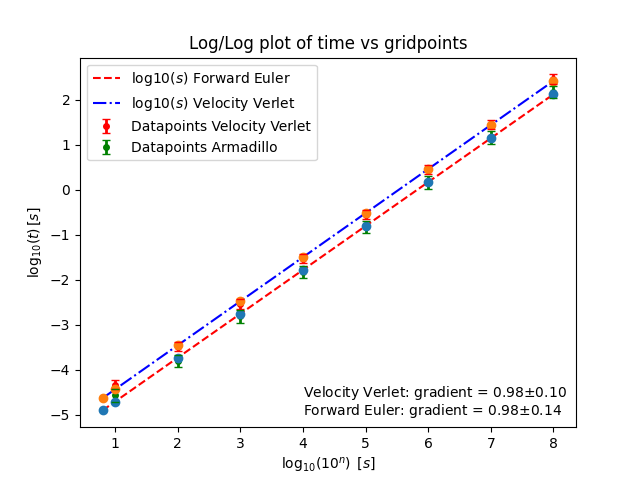
\includegraphics[width=0.9\linewidth]{../code/classes/figure/TC.png}
	\caption{Plot of the run time for forward Euler versus the velocity-Verlet method. Data points chosen are also plotted including error bars for the maximum deviation from the best fit line, found by using least squares method. Seen is that velocity-Verlet method is overall slower than forward Euler, however both methods follow linear scaling.}
	\label{fig:TC}
\end{figure}
\begin{figure}[]
	\centering
	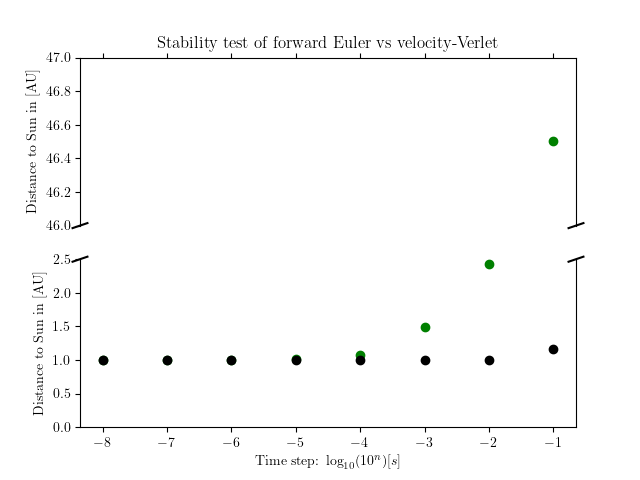
\includegraphics[width=0.9\linewidth]{../code/classes/figure/Stability.png}
	\caption{Plot of the relation between the time step and final position of the Earth in AU from the Sun. Green points are from the forward Euler algorithm, whilst the black points are from the velocity-Verlet algorithm. We see that at $n = -5$ that the distance of from the Sun for both algorithms coincide. There are no data from $n<-8$ as the run time of the program starts getting exponentially high.} 
	\label{fig:Stability}
\end{figure}
\subsection{Two-Body System}%1
We see the results for calculating the movement of the Earth-Sun system over a century in figure \ref{fig:FE} and figure \ref{fig:VV}. We see for the velocity-Verlet algorithm in figure \ref{fig:VV}, that we have a stable orbit with little to no visible wobble. Looking at the plot from the forward Euler algorithm in figure \ref{fig:FE}, we see that the algorithm does not provide a good prediction of the motion of the Earth, there is a gradual increase in the radial distance to the Sun.

\begin{figure*}[t]
	\centering
	\begin{subfigure}{9cm}
			\centering
		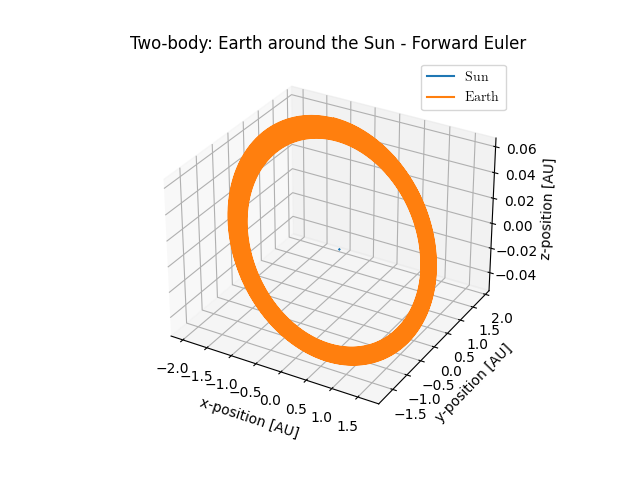
\includegraphics[width=9cm]{../code/classes/figure/ESFE.png} 
		\caption{Earth-Sun system plotted over 100 years using the forward Euler algorithm. We see a clearly visible increase in the distance to the Sun,.}
		\label{fig:FE}
	\end{subfigure}%
	\begin{subfigure}{9cm}
			\centering
		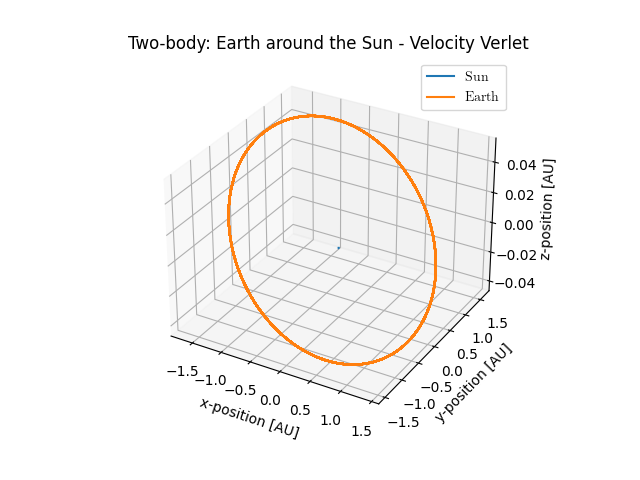
\includegraphics[width=9cm]{../code/classes/figure/ESVV.png}
		\caption{Earth-Sun system plotted over 100 years using the velocity-Verlet algorithm. We see a even orbit around the Sun, with no visible difference in the radial distance between the Earth and the Sun.}
		\label{fig:VV}
	\end{subfigure}
	\caption{Plot of the Earth-Sun system over 100 years, using a time step of $10^{-4}$years for both plots. Initial conditions are from NASA, using the Sun as center of mass.}
	\label{fig:2B}
\end{figure*}
\subsection{Change of Force}%1

In the figures \ref{fig:Ca} and \ref{fig:Ea} alpha denotes 
\begin{equation}
	F_G \propto \frac{1}{r^{\alpha}}
\end{equation}
which is the current value of Newton's gravitation force we testing. 
Important to note for this test, is that we are using double precision numbers for the power, meaning that our values may not always be completely accurate to the value wanted.

Looking at the simulation with Earth's initial orbit given as $2\pi$, which results in a circular orbit we can see from figure \ref{fig:Ca}, that for values of $\alpha \geq 3$, that the orbit becomes unstable. It can be seen at the tail end of the simulation around 300 years, that for $\alpha = 3$, we can see what could resemble an unstable orbit.  

Looking at the simulation for the elliptical orbit in figure \ref{fig:Ea}, we see the same behavior as for the circular orbit. As soon as $\alpha > 3$, the Earth escapes orbit. 
\begin{figure*}[t]
	\centering
	\begin{subfigure}{9cm}
		\centering
		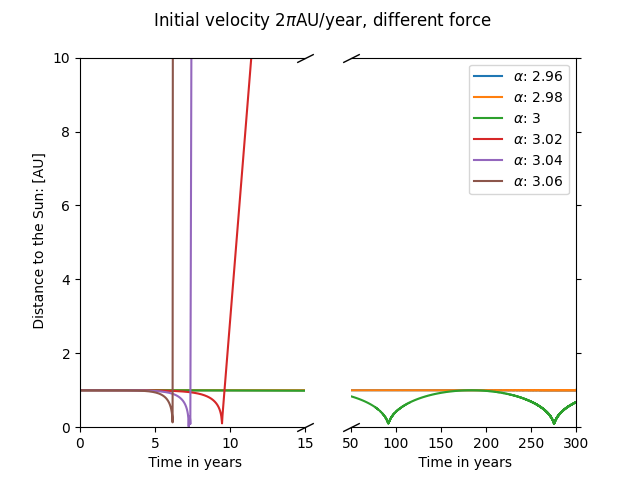
\includegraphics[width=9cm]{../code/classes/figure/ForceCirc.png} 
		\caption{Plot over the radial distance from the Earth to the Sun, compared to different values of the $\alpha$. We see that even for $\alpha = 3$ the Earth does not escape orbit as it does for higher values of $\alpha$. The axis are split as the motion of the Earth as soon as it becomes unstable, is very sudden. We see that for the higher values of $\alpha$ the Earth rockets our of orbit around the Sun within 10 years.}
		\label{fig:Ca}
	\end{subfigure}%
	\begin{subfigure}{9cm}
		\centering
		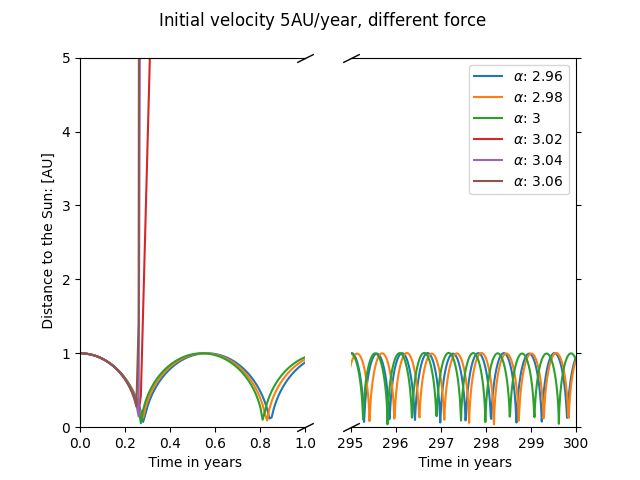
\includegraphics[width=9cm]{../code/classes/figure/ForceElip.png}
		\caption{Plot over the radial distance from the Earth to the Sun, compared to different values of $\alpha$. A similarly high step for the chosen values of $\alpha$ is chosen here. We see a similar behavior for for the orbit until $\alpha > 3$.}
		\label{fig:Ea}
	\end{subfigure}
	\caption{The Earth-Sun system simulated with different variants of Newton's gravitational force. For circular orbit, and elliptical orbit.}
	\label{fig:Force}
\end{figure*}
\subsection{Escape Velocity} %1 
Through trial and error we found that for our program the numerical escape velocity of the Earth starting at 1 AU from the Sun is, to four decimal places $\vec{v}_{\text{escape}} = 8.8849$ AU/year, which is less than the analytical value of $2\pi\sqrt{2} \approx 8.8858$\footnote{To four decimal places.}, this is a relative deviation of 0.01$\%$.
\subsection{Three-Body System}%1
Looking at our plots of the three body system in figure \ref{fig:ThreeBody} we have four different plots. Figure \ref{fig:TB1}, \ref{fig:TB10} and \ref{fig:TB1000}, are our plots using the Sun as the center of mass and changing the mass of Jupiter. Whilst figure \ref{fig:TBJE} is using the center of mass of the three body system, using data from NASA. We see that using the Sun as the center of mass and using the center of mass of the three body system, creates similar orbital patterns with no notable difference, this is due to the massive difference in mass between the Sun and, the Earth and Jupiter. The center of mass lies just outside the surface of the Sun for the three body system, so we would actually expect equal orbits. 

Looking at figure \ref{fig:TB10} where we have increased the mass of Jupiter by a factor of 10, we see a noticeable effect of the gravitational pull of Jupiter on both the Sun and on Earth, where Earth's orbit around the Sun, is shifted along side the Sun, closer to where Jupiter is located in its orbit. If we ran the simulations over a longer time period, we could expect our system to orbit around a shifted center of mass. 

For our last simulation we increased Jupiter's mass by a factor of 1000, the results of this can be seen in figure \ref{fig:TB1000}. Here we see the clear effect of Jupiter's gravitational pull on both the Sun and Earth. The mass center in this case would lie roughly in the middle between the Sun and Jupiter, and we see preface of a spiral orbit for the Sun and Jupiter in the bottom right corner. We also see that the Earth is slung around Jupiter out of orbit. 

\begin{figure*}[t]
	\centering
	\begin{subfigure}{9cm}
		\centering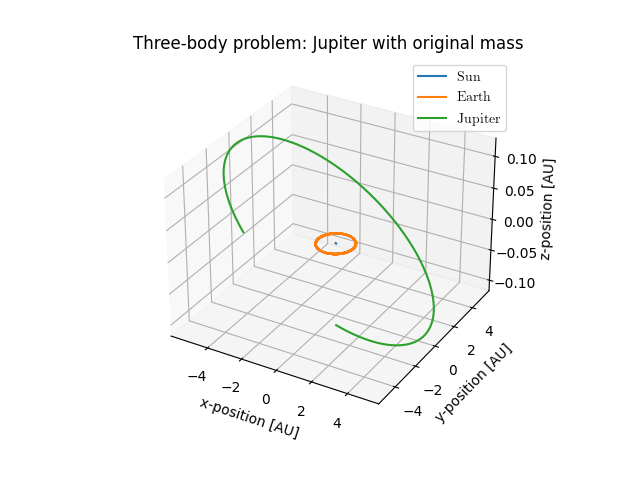
\includegraphics[width=9cm]{../code/classes/figure/TB1.png}
		\caption{Plot of three-body system with Jupiter's original mass of Jupiter over 10 years, with a time step of 52.6 minutes or $10^{-4}$years. The Sun is set to initial position is the origin with no initial velocity. We see that the Earths motion resembles that of a circular orbit, with possibly minor deviations, not visible in the plot. }
		\label{fig:TB1}
	\end{subfigure}%
	\begin{subfigure}{9cm}
		\centering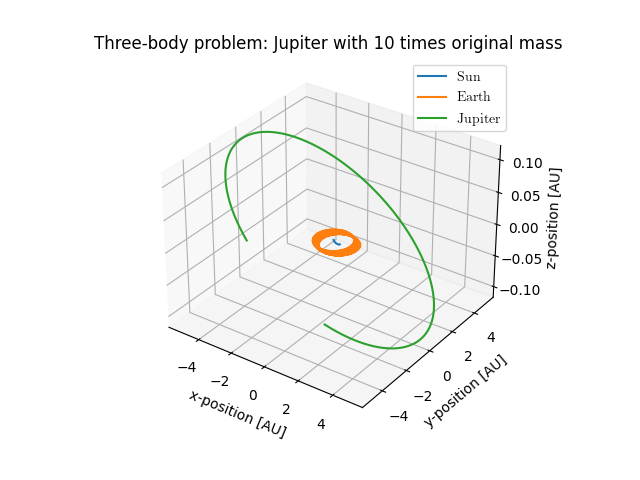
\includegraphics[width=9cm]{../code/classes/figure/TB10.png}
		\caption{Plot of three-body system with Jupiter's 10 times the original mass of Jupiter over 10 years, with a time step of 52.6 minutes or $10^{-4}$years. The Sun is set to initial position is the origin with no initial velocity. We see that Earths motion wobbles and see what resembles a greater attraction of the Earth towards Jupiter, the same can be seen in the position of the Sun. This is expected from an factor of 10 increase in the force acting on the Sun and Earth from Jupiter.}
		\label{fig:TB10}
	\end{subfigure}\vspace{10pt}
	
	\begin{subfigure}{9cm}
		\centering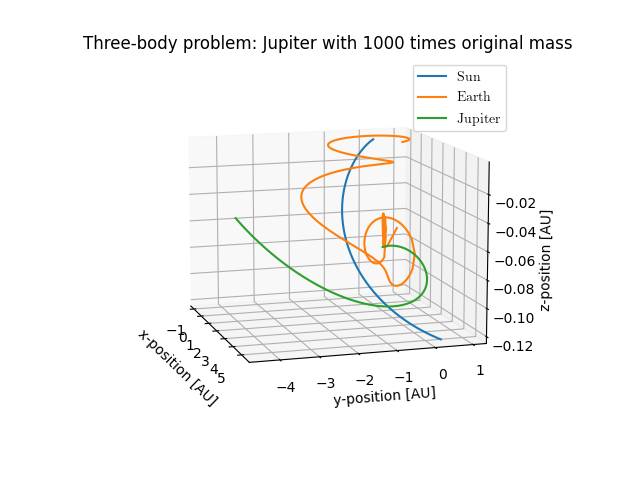
\includegraphics[width=9cm]{../code/classes/figure/TB1000.png}
		\caption{Plot of three-body system with Jupiter's 1000 times the original mass of Jupiter over 10 years, with a time step of 52.6 minutes or $10^{-4}$years. The Sun is set to initial position is the origin with no initial velocity. Here the Earth eventually get slingshot out of orbit around Jupiter, and what could be seen at later stages is that the Earth escapes orbit around both planets. Also we see what could potentially be a spiral orbit of the Sun and Jupiter.}
		\label{fig:TB1000}
	\end{subfigure}%
	\begin{subfigure}{9cm}
		\centering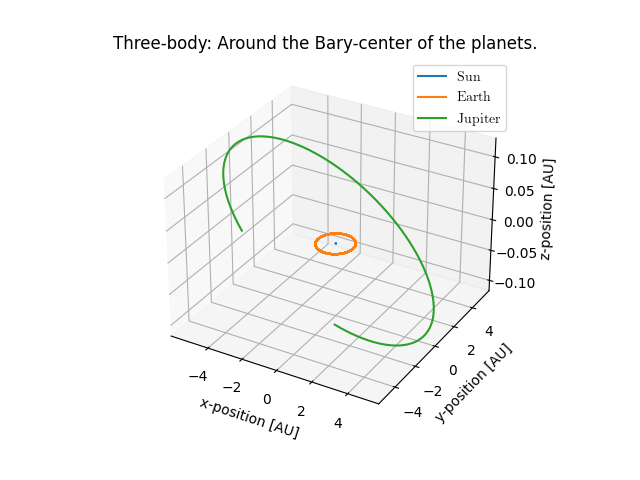
\includegraphics[width=9cm]{../code/classes/figure/TBB.png}
		\caption{Plot of the three-body system where we use data from NASA and shift the center of mass of the system to be the actual center of mass of the system. Included we choose the initial velocity of the Sun such that the total angular momentum of the system is zero. Plot is over 10 years with a time step of 52.6 minutes or $10^{-4}$years.}
		\label{fig:TBJE}
	\end{subfigure}
	\caption{Plots of the three-body problem.}
	\label{fig:ThreeBody}
\end{figure*}

\begin{figure}[]
	\centering
	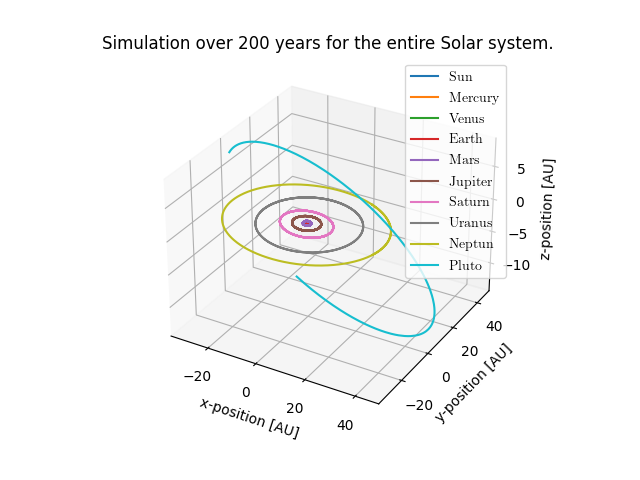
\includegraphics[width=0.9\linewidth]{../code/classes/figure/SS10.png}
	\caption{Simulation of the entire Solar system over two centuries. See also plot over the inner planets.}
	\label{fig:SS10}
\end{figure}
\begin{figure}[]
	\centering
	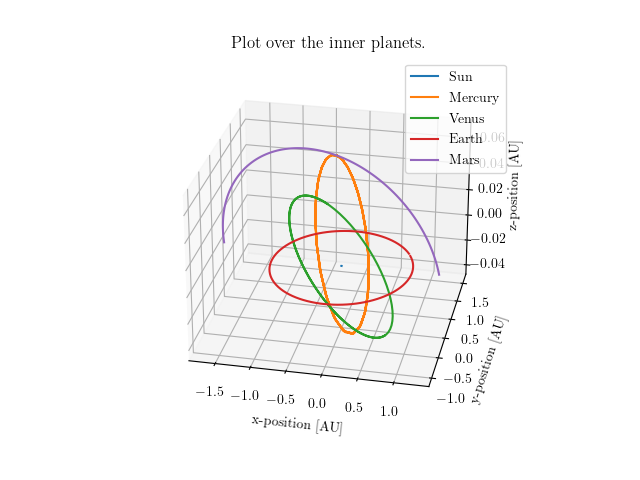
\includegraphics[width=0.9\linewidth]{../code/classes/figure/InnerPlanets.png}
	\caption{Plotting the inner planets motion over two centuries results in unreadable data due to their short orbits, whilst for the outer planets, we can see for some, only partial orbits.}
	\label{fig:IP}
\end{figure}
We also see from our simulation of the entire Solar system seen in figure \ref{fig:SS10} that all the planets seems to follow stable orbits. This also goes for the plot over the inner planets in figure \ref{fig:IP}, where we have stable orbits and the Sun seems to be fixed to the center of the system. 

\subsection{Perihelion Precession of Mercury}%1
In figure \ref{fig:PP} we see the different perihelion precession of Mercury shown in arc seconds from the initial position given by the first perihelion at 0''. The annotated value is our prediction of the perihelion precession using the data from our 10 year simulation with a time step of $10^{-8}$ years, to predict the final value, to three decimal places, after a century. This is supported by our found value for a simulation over a century with a time step of $10^{-7}$years to three decimal places. The predicted difference between the two values is 43'', so our results are 0.388'' away from the predicted results. 
\begin{figure}[]
	\centering
	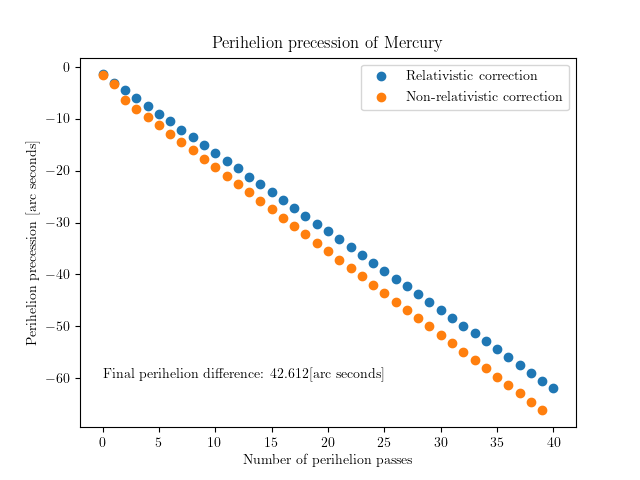
\includegraphics[width=0.9\linewidth]{../code/classes/figure/PP.png}
	\caption{Plot over the perihelion precession of Mercury in a system containing only Mercury and the Sun. Data is shown in the movement of the perihelion from the initial position of 0''. The data sets are from simulation using both a relativistic correction and no relativistic correction, both over a 10 with time step of $10^{-8}$ years.}
	\label{fig:PP}
\end{figure}


\section{Discussion} %1
\subsection{Center of Mass} % 1
As we saw in the data earlier, not fixing the center of mass of our systems to the center of the Sun, absolutely, that is that Sun has zero degrees of freedom, has little to no effect on our numerical data in most cases. For both our two-body system and three-body system, the actual center of mass is at largest just outside the surface of the Sun\cite{1994A&A...282..663S}, which amount to roughly $0.004655$AU. 
However when looking at the effects of Jupiter's gravitational force on Earth, with masses of 10 times and 1000 times its original mass, we saw that the Sun's position not being absolutely fixed, but having free motion. We observe that Jupiter's increase in mass not only effects the Earth, but also the Sun is forced into motion, around a shifted center of mass. As Jupiter is approximately 1000 times lighter than the Sun, when we increase the mass of Jupiter by a factor of 1000, we would have a shifted center of mass, which would lie just in the middle between The Sun and Jupiter. 
In these two cases we would expect different results if we give the Sun zero degrees of freedom, or free movement.

\subsection{Stability and Time} %1
For the simple test of the Earth-Sun system, we can see a clear difference in how the velocity-Verlet algorithm and the forward Euler algorithm performs. From figure \ref{fig:FE} we see that the forward Euler, creates a significant change in the orbit of the Earth. Where we orbit seems to increase and the Earth slowly drifting away from the Sun, if compared the the velocity-Verlet algorithm in figure \ref{fig:VV}. Here we see a stable orbit with a constant distance between the Earth and the Sun, this is the result we would expect if energy is conserved. Whilst for the forward Euler, where energy is not conserved we see that the total energy in the system is not constant and the Earth drifts further and further away. If we simulated over a long enough period, we could expect that the Earth eventually escapes orbit, when the radial distance to the Sun gets large enough as the force acting from the Sun on the Earth gets gradually smaller. 

Seen from figure \ref{fig:Stability} we can see that for $n = -4$, that we actually have a slight difference between the velocity-Verlet algorithm and the forward Euler algorithm. The results of the orbits could be different if a smaller time step would have been chosen, but for longer simulations using a small time step would be time sensitive. Also in the grand scheme of things, we would prefer to be able to run our simulations over many years without having too long of a run time. 

Looking at figure \ref{fig:Stability} again, we have a clearly better choice in the velocity-Verlet algorithm, as it produces more accurate results with less time steps. This in turn makes us able to simulate a system of longer time periods quickly, however even whilst the algorithm is stable, we would not expect extremely precise results when choosing a large time step, but we can be fairly sure when choosing the velocity-Verlet algorithm, that we would not get solutions which are completely unrealistic from a macro perspective. 

Important to note is that FLOPs is not a direct measurement of run time, but gives an indication of how long one algorithm will run compared to another. In our case with the forward Euler and velocity-Verlet, the forward Euler needs a factor of 2, less FLOPs than velocity-Verlet, which is supported by run time test. This could be by coincident, but the relation that the velocity-Verlet algorithm should have a longer run time is supported. 

Even though we have a trade off in time usage, the notable advantage of using the velocity-Verlet out weights the minor increase in run time. Having an algorithm that preserves both angular momentum and total energy when working with physical systems is key to be able to analyze them correctly. 

\subsection{Change of Force} %1
When studying different values for $\alpha$ in the force, we see that the behavior of the orbit changes as $\alpha$ approaches 3. Most importantly to note here is the change in behavior we see as soon as $\alpha > 3$, where for both cases of initial velocity we see that the Earth escapes orbit. We see that even for $\alpha = 3$, that the orbit remains stable, however as we are using double precision numbers for $\alpha$. The actual values used for the exponent could be smaller or larger than intended. This would lead to contaminated results, where our simulation would create false results. This would in that case be a problem with our method. 
It would be better to simulate $\alpha = 3$ using an integer value instead, or use a finer granulation of increments when studying $\alpha$. 

One implication of this, is that when studying $\alpha = 3$ with, initial velocity $2\pi$, we see that the orbit starts fluctuating a lot. As this is a double precision number, we would expect it to not be $3$, however just slightly short of 3. 
From this one could deduce that for $\alpha = 3$, we could reasonably expect the Earth to leave orbit. However we do not have any results to back this claim up for our simulations, which is a major downside. 

So running the simulations again with finer increment of $\alpha$ and a smaller time step, we could end up with a better results of what happens just as $\alpha$ approaches 3. 
Even though the evidence is clear, that the Newtonian gravitational law, could not sustain stable orbits if $\alpha > 3$. 
\subsection{Escape Velocity} %1
For finding the escape velocity, as we have an analytical solution, we can quickly narrow down the range of value we want to search in. However there are two major problems when trying to find the escape velocity of a planet orbiting around a star numerically. How long do we need to iterate to be sure the planet is no longer in orbit? How far away does the planet need to be to no longer be in orbit? Essentially one would need to approximate infinity in both cases which is not feasible. Here we chose to approximate the time period with 5000 years and the distance away from the Sun, to classify the Earth as escape to 100 AU.

When comparing our result to the analytical answer, we can see that we are within $\sim 0.0009$ AU/year to the actual value. This is $\sim 153.6$km/h, which in the grand scheme is not a large value. We could have gotten a closer approximation with changing how we define the maximum time, escaped distance and our time step. But ultimately we are at the mercy of what computers are capable of, and a difference in $153.6$ km/h or roughly $42$ms/s when shooting blindly at different velocities is a okay result. 

One improvement which could have been done, is rather than trying to find the escape velocity through simulations of the system, rather find it through root finding, similar to the method used to find the analytical result. 
\subsection{Three-Body system} %1
Studying the three body system we see how a large object affect Earths orbit around the Sun. Looking at our two first simulations, seen in figures \ref{fig:TB1} and \ref{fig:TBJE}, we see similar orbits with no noticeable difference in the orbits. When finding the center of mass of the two systems it is found to lie just outside the surface of the Sun. This indicates that simulating this system, with the center of mass placed at the center of the Sun, is not a bad starting point. We would not get the correct simulation, but for an overall perspective it is a fair assumption to make as commented earlier. 

Studying the cases where we change the mass of Jupiter we see very different motion of our system, which is supported if we consider the center of mass. For the case where we increase the mass of Jupiter by a factor of 10, we see the orbit of the Earth around the Sun, follows where Jupiter is located in its orbit. Over a longer simulation we would expect the entire system, if stable, would orbit around the common center of mass. We also see that the Sun is put into noticeable motion, by the increase in Jupiter's mass. Not too surprising as Jupiter is roughly a factor of 1000 lighter than the Sun, so we are introducing two Sun-like objects into our three body system. 

If we had initialized our system, with co-planar motion between the Sun and Jupiter we would see the spiral or circular motion of the two Sun-like objects around their common center of mass, however now predictions of the motion of the Earth is made, as we have no data to predicts its motion. 


For our simulation of the entire Solar system we can see that all orbits are stable and the same goes for the plot over the inner planets, which is hard to decipher from the large scale plot. The orbits seems to be stable, and the Sun fixed in the middle. We would expect some motion of the Sun as the center of mass would be located outside the center of the Sun, and as seen in figure \ref{fig:SS10}, we see that inside the orbit of Mars the orbits seems to over lap a bit. This is because the center of mass of the entire system would shift as the system evolves, thus altering the orbits of the inner planets more significantly than those of the outer planets. Plotting the motion of the inner planets for the entire simulated time period, would only result in an unreadable plot, as the orbits would shift as the system evolves. However we see no planets leave orbit and for the shorter time all orbits seems to be stable, so we can assume that the orbits would remain stable for the entire simulation.
\subsection{Perihelion Precession of Mercury} %1
Studying the perihelion precession of Mercury, the test for general relativity, we find that our numerical results seen in figure \ref{fig:PP} are close to the observed values of the perihelion precession. The perihelion precession of Mercury, is so small, that one would need a small time step to be able to notice it. However to three decimal places, we have found that we get not difference between our methods of finding perihelion precession. 

Essentially the perihelion precession is a linear change, as we can see from figure \ref{fig:PP}, and thus we can predict to how large this value should be after a certain time period. However as with any numerical method goes, we are limited by numerical precision for finding this value to a high accuracy. One way of finding this value to a high accuracy would be to lower the time step to a smaller value, however when simulating over a long period of time, we would quickly run into run time problems, for normal computers. For the stability looked at in this project we had chosen a maximum value for $n = -8$, this would entail that we have no data if we make the time step smaller. From previous studies of numerical precision we know that if the time step gets too small the error increases, which would not be different in this case. 

As this is an effect which is normally observed over a century, we would like to run our simulations for the same time period, but as said, with a small enough time step, this is computationally expensive and not feasible. An approach to this, knowing how the perihelion precession changes, we can adapt our methods and rather than doing simulations over a century, choose a shorter time period and rather a smaller time step to simulation Mercury's position precisely. 

This is done in this project, and as noted we did not find any difference to three decimal places, however one may expect if considering enough significant figures, we would observe a difference in the two methods. One has to choose what is most important in this case, computational time or precision in the results. As we do not have access to any super computers it is safe to say, that computational time is a limiter and we would rather have results that are fairly accurate, than as of writing this, still be computing the perihelion precession. 

An improvement that could have been made is using data from NASA to initialize the system and using the center of mass to the actual center of mass of the Mercury-Sun system instead of the Sun as the center of mass. This could lead to more precise results, however a standard deviation of $0.9\%$ is within reason for the setup of our simulation. 
Thus we can conclude that the perihelion precession of Mercury can be at least partially explained by general relativity. There would in the real world case, be a multiple factors which affect the orbit of the planets, even small things like absorption of light would affect the orbits of all the planets. However these effects are so small, that if our numerical results are accurate, the majority of the perihelion precession of Mercury can be described by general relativity. 

\subsection{Object Orientation and Memory} %1
Object orientation removes a lot of the head ache when needing to include large amount of objects into systems you want to solve. Also here having object oriented code remove a fair bit of headache, whilst also creating some. To choose one programming paradigm over another, is not just bonuses, they all come with their own downfalls. Specifically for object orientation, it is within the idea of writing your code as general as possible, whilst still being easy to read, encapsulated and able to solve the problems at hand. In this project some of the design problems comes from how we calculate the force acting on an object. Since we are interested in three different cases for how the force is calculated, namely, Newton's gravitational law, adaptation of Newton's gravitational law and relativistic correction. We have three different ways to calculate the force, and how one should approach this may differ. 
You want to have a solver class which can adapt to each of the different force, without actually needing to change. Here our solution in the C++ implementation is to assign the varying part of the force when initializing the Solar system, and keeping our solver general. 

Whilst our approach to memory is good for large systems, especially if the number of iterations gets large, writing the data to a file for every k iteration also has its downsides. We effectively shift our resource usage from the memory to the CPU and if the number of points we write is large enough this could cause issues. 
One could in the cases for relatively low number of integration points adapt pseudo multi dimensional arrays, to gain a further speed up, but at the cost of memory. There are many different data structure approaches to this problem, all with their own upsides and downsides, so you can pick and choose what method one think would work best for the problem at hand. 
\section{Conclusion} %1
When studying the Solar system, and studying the orbits of the planets, we end up having to solve systems of coupled differential equations. By discretizing the continuous equations and using natural units to scale them, we can reproduce analytical results and solve analytically unsolvable problems. Using the results we are able to compare two algorithms, forward Euler and velocity-Verlet. Both total energy and angular momentum should be conserved when we study the Solar system. We found from the two-body system that the velocity-Verlet algorithm reproduces the orbits of the planets more accurately, even when adding more planets to the system than the forward Euler. In addition, we found that the velocity-Verlet algorithm preserves total energy and angular momentum compared to the forward Euler, as mentioned this was implemented as a unit test. 
The only downside to using the velocity-Verlet algorithm compared to forward Euler is the run time, having a factor of 2, FLOPs more, resulting in twice the run time. But is still superior due to its accuracy. 

We studied two interesting areas for the two body system, namely escape velocity and altering Newton's gravitational law. 
When trying to numerically approximate the escape velocity we found has a relative deviation from the analytical value of $0.01\%$, which is good for a shooting blind method of simulating the system. In the future using root finding algorithm to find the escape velocity would be a better way of getting closer to the analytical value, as simulating the system is at higher risk of loss of numerical precision, if the time step gets too small, which would be preferable when trying to find precise values. 
Studying the alteration of Newton's gravitational law, we find that both systems appear to be stable up until $\alpha = 3$, as mention since the values where stored as double precision digits, the actual value of $\alpha$ would not be exact equal to 3. This could lead to wrong results for the noted values of $\alpha$, however we can deduce that for $\alpha > 3$, that the system is no longer stable. 
In addition, some instabilities could be seen when the number of iterations becomes large, when $\alpha$ approaches three. 

Studying the three body system of Earth, the Sun and Jupiter, for different masses of we found saw some interesting motion of both the Earth, and the interacting between the Sun and Jupiter. 
For the cases where we studied Jupiter with its original, only using different center of mass, we saw the the orbits where indistinguishable from each other for the simulation period. Making our assumption for the center of mass seem correct, especially for shorter simulations. 
When studying increased mass of Jupiter we found clear signs in the orbits that the center of mass is no longer close to the origin, and the orbits starts to deviate from the normal orbits. For the case where Jupiter's mass is 10 times its original mass, we still see that the system seems to be stable, but as soon as we increase the mass to 1000 times the original mass, we have an unstable system. The Earth is slung our of orbit and the Sun and Jupiter starts orbiting each other. 

We also looked at the perihelion precession of Mercury and found that the value we found numerically for the perihelion precession was 42.612'' which was backed up by two different simulations. From which we can deduce that the perihelion precession of Mercury at least can partially be explained by general relativity. This is a relative deviation from the observed result of $0.9\%$, which including the additional factors affecting Mercury's orbit, our findings can be considered accurate. 

Lastly adapting an object oriented style for the code base, makes us able to adapt our problem to any number of objects. We could create a full model of the entire Solar system, without having to make any adaption to the code base. This is a big upside to the object oriented style of coding, whilst it has its limitation if following all the object orientation paradigms, we can still create functional code which has a good structure and easy adaptability.

\bibliography{bib_proj3}
\bibliographystyle{plain}


\end{document}
